\documentclass[12pt]{article}

\usepackage{sbc-template}
\usepackage{graphicx,url}
\usepackage{listings}
\usepackage{longtable}

\usepackage[brazil]{babel}   
%\usepackage[latin1]{inputenc}  
\usepackage[utf8]{inputenc}  
% UTF-8 encoding is recommended by ShareLaTex

     
\sloppy

\title{Algoritmo genético para cálculo da tabela de horários dos Componentes Curriculares do curso de Ciência da Computação da UFFS}

\author{Gabriel Batista Galli\inst{1}, Matheus Antonio Venancio Dall'Rosa\inst{1}, Vladimir Belinski\inst{1}}

\address{Ciência da Computação -- Universidade Federal da Fronteira Sul
  (UFFS)\\
  Caixa Postal 181 -- 89.802-112 -- Chapecó -- SC -- Brasil
  \email{\{g7.galli96, matheusdallrosa94, vlbelinski\}@gmail.com}
}

\begin{document} 

\maketitle
     
\begin{resumo} 
  O presente trabalho, apresentado ao curso de Ciência da Computação da Universidade Federal da Fronteira Sul - UFFS - Campus Chapecó - como requisito parcial para aprovação no Componente Curricular Inteligência Artificial, 2017.1, sob orientação do professor José Carlos Bins Filho, consiste em uma descrição detalhada da implementação de um algoritmo genético para calcular a tabela de horários dos Componentes Curriculares do curso de Ciência da Computação da UFFS.
\end{resumo}

\section{Descrição geral do algoritmo}

A implementação do algoritmo genético encontra-se distribuída em dois arquivos: \emph{main.cpp}, o arquivo principal, cujo conteúdo engloba as funções do programa; e \emph{ia.h}, o arquivo de cabeçalho de \emph{main.cpp}, onde se encontram declaradas as estruturas utilizadas e alguns protótipos de funções.

O fluxo de execução do algoritmo pode ser encontrado na função \emph{main()} de \emph{main.cpp}. Inicialmente, realiza-se uma chamada à função \emph{read\_professors()}, que realiza a leitura dos professores e horários que não desejam ministrar aulas, a partir do arquivo de entrada.

Em sequência é calculada a \textit{fitness} máxima de um indivíduo, dada da seguinte maneira: inicia-se com uma \textit{fitness} de $450$ pontos, dos quais $30$ consistem em pontos atribuídos ao professor pelo fato dele não estar dando aula nos horários que não deseja, $30$ pelo fato de não estar dando aulas nos períodos matutino e noturno no mesmo dia, $30$ por não estar dando aulas sequenciais e $360$ por não estar dando aula no último horário de uma noite e primeiro do dia seguinte. Os três primeiros casos se relacionam às preferências estabelecidas na descrição do trabalho proposto e o último corresponde à última restrição elencada. Cabe destacar que, devido a maneira em que o algoritmo foi implementado, as demais restrições não são violadas.

Ao ser realizada uma violação da preferência que nos informa que um professor não deveria dar aula nos horários que não deseja, é realizado um desconto de $1$ ponto por horário infringido (dentro de um limite de $30$ possíveis horários de uma semana, motivo pelo qual a \textit{fitness} do indivíduo inicia com $30$ pontos atrelados a essa preferência). Por sua vez, ao ser violada a preferência que indica que um professor não deveria dar aula nos turnos matutino e noturno no mesmo dia, é realizado um desconto de 6 pontos na \textit{fitness} do indivíduo por dia infringido (são $6$ pontos, pois temos inicialmente $30$ pontos para essa preferência e cinco dias na semana. Logo, $30 / 5 = 6$). Adicionalmente, ao ser realizada uma violação da preferência que apresenta que um professor não deveria dar aulas de maneira sequencial (um turno inteiro), é realizado um desconto de $2$ pontos por turno infringido (são 2 pontos, pois temos inicialmente $30$ pontos para essa preferência e $15$ possíveis casos de aulas sequenciais por semana. Logo, $30 / 15 = 2$). Às três preferências foram atribuídos $30$ pontos iniciais para que, assim, elas possuíssem o mesmo peso no cálculo da \textit{fitness}.

Por fim, a restrição que informa que um professor não pode dar aula no último horário de uma noite e no primeiro horário da manhã seguinte é levada em conta na função de \textit{fitness} da seguinte forma: inicialmente são atribuídos  $360$ pontos na \textit{fitness} de um indivíduo para a não violação dessa restrição. A cada infração dela $90$ pontos são descontados da \textit{fitness} do indivíduo (são $90$ pontos, pois temos $360$ pontos iniciais e $4$ possibilidades de violação -- $(21,02)$, $(23,04)$, $(25,06)$, $(27,08)$. Logo $360 / 4 = 90 $). São $360$ pontos para a restrição, pois, como uma violação de restrição não deve ocorrer, foi decidido que $80\%$ da \textit{fitness} seria atribuída a ela, de maneira que indivíduos que tivessem a restrição violada (caso com poucas ocorrências nos testes realizados) sofressem significativas penalidades e consequentemente tivessem sua probabilidade de reprodução amplamente diminuída.

Devido ao fato de não ter sido utilizado números de ponto flutuante para a representação da \textit{fitness} e a fim de ser mantida a proporcionalidade de um valor entre $0$ e $1$, multiplicamos o valor inicial máximo da \textit{fitness} explanado acima pelo número de professores dado na entrada.

Em seguida, é calculada a \textit{fitness} máxima da população, dada pela multiplicação da \textit{fitness} máxima de um indivíduo pelo tamanho da população.

Cabe enfatizar que as funções relacionadas ao cálculo da \textit{fitness} de um indivíduo, de uma população e de suas penalidades são, respectivamente, \emph{fitness()}, \emph{set\_population\_fitness()}, \emph{count\_schedules\_to\_avoid\_infringements()}, \emph{count\_mo- rning\_night\_infringements()}, \emph{count\_consecutive\_schedules\_infringements()} e \emph{count\_re- striction\_infringements()}, todas presentes em \emph{main.cpp}.

Sequencialmente, são lidos do arquivo de entrada os cursos/semestres, salas e horários disponíveis para a salas (função \emph{read\_room\_schedules()}) e os CCRs, períodos, cursos/semestres e professores (função \emph{read\_subjects()}).

Após isso, é realizada a geração da população inicial, armazenada na estrutura \emph{population\_t} e montada através da chamada das funções \emph{generate\_people\_permutation()} e \emph{generate\_population()}.

Na função \emph{generate\_people\_permutation()} é realizada a construção de $m$ permutações aleatórias, sem uso de \textit{backtracking}. Seja $Professors = \{p_{1}, p_{2}, . . . , p_{m}\}$ o conjunto de professores recebidos na entrada, e uma permutação $P_{i}$ definida por $P_{i} = \{p_{i_{1}}, p_{i_{2}}, . . . , p_{i_{m}}\}$, é feito $p_{i_{1}} = p{1}$ e sorteados os $m-1$ professores restantes sem uso de \textit{backtracking} para as posições $\{p_{i_{2}}, . . . , p_{i_{m}}\}$ da permutação $P_{i}$.

A construção dos indivíduos (com tamanho igual ao parâmetro constante \textsc{population\_size}) acontece da seguinte forma: a população é dividida em $m$ grupos de tamanho $g = \textsc{population\_size} / m$. Um grupo $m_{i}$ é construído a partir da permutação $i$, ou seja, a primeira permutação de $m_{i}$ é $m_{i_{1}} = P_{1}$. Então, são geradas $m-1$ permutações lexicograficamente ordenadas a partir da permutação $P_{i}$, sendo utilizado para tal o algoritmo implementado na função \emph{next\_permutation()} da biblioteca \emph{algorithm}. Cabe destacar que cada indivíduo é construído a partir de uma permutação.

Seja $schedule_{i}$ um par sala e horário, e $schedules$ um conjunto de pares de sala e horário, o conjunto $schedules$ é ordenado de tal forma que $schedule_{i} < schedule_{j}$ e $i < j$, caso a sala de $schedule_{i}$ possua menos horários disponíveis do que a sala de $schedules_{j}$. Dada a ordenação apresentada, à cada indivíduo é realizada a atribuição de seus horários, sendo esses tomados de maneira sequencial a partir de $schedule_{1}$.

Finalmente, é realizada uma chamada à função \emph{evolve()}, que recebe como parâmetro a quantidade de gerações em que o algoritmo será executado e é responsável pela evolução da população. A cada geração uma nova população é inicializada, sendo os indivíduos dessa nova população resultantes do cruzamento de dois indivíduos da população atual, que, por sua vez, são sorteados de maneira com que os indivíduos que apresentem maior \textit{fitness} tenham maior probabilidade de reprodução. São realizados cruzamentos até que a nova população atinja o tamanho da atual. Após cada cruzamento (detalhado na seção ``Cruzamento dos indivíduos'') é realizada a mutação do indivíduo resultante dentro de uma probabilidade especificada no código (a mutação será detalhada na seção ``Mutação dos indivíduos'').

Ainda a respeito da implementação do algoritmo, cabe destacar os critérios de parada estabelecidos para esse. O algoritmo é finalizado quando ocorre um dos seguintes casos:

\begin{enumerate}
    \item Quando é gerado um indivíduo de \textit{fitness} máxima, ou seja, uma resposta ideal/perfeita ao problema, na qual não haveria nenhuma violação de restrições e preferências;
    \item Quando a \textit{fitness} de uma população se mantém inalterada por um número estabelecido de gerações, definido no parâmetro constante \textsc{max\_unmodified\_generations};
    \item Quando o algoritmo atinge um número máximo de gerações, definido no parâmetro constante \textsc{max\_generations}.    
\end{enumerate}

Cabe destacar que ao longo da execução do algoritmo são impressas no console a numeração das gerações, a \textit{fitness} de sua população e a \textit{fitness} máxima. Ao ser atingido um dos critérios de parada informados, também é destacado por qual motivo a execução foi finalizada e impressos no console os dados do indivíduo de maior \textit{fitness} da última população gerada. Por fim, cabe destacar que para fins de debug pode ser descomentado o define de debug no arquivo \textit{main.cpp}, o qual faz com que sejam impressas mais informações no console durante a execução do algoritmo.

\section{Representação de um indivíduo}

Um indivíduo é representado pela estrutura \emph{person\_t}, presente em \emph{ia.h}, sendo definido por uma lista de genes e um valor de \textit{fitness}.

Por sua vez, cada gene é representado pela estrutura \emph{schedule\_t}, presente em \emph{ia.h}, que armazena as informações referentes à sala de aula (estrutura \emph{room\_t}, que contém o número da sala, o curso e os horários disponíveis da sala), ao componente curricular (estrutura \emph{subject\_t}, onde também pode ser encontrado, por exemplo, o professor associado ao componente curricular e o curso), ao horário da semana e o número do período.

\section{Cruzamento dos indivíduos}

A implementação do cruzamento pode ser encontrada na função \emph{cross()} de \emph{main.cpp}. A chamada de \emph{cross()} é realizada dentro de \emph{evolve()}, de forma a gerar os indivíduos de uma nova população. \emph{cross()} recebe como parâmetros um indivíduo pai e um indivíduo mãe, sorteados da forma apresentada na seção ``Descrição geral do algoritmo''.

Inicialmente, são agrupados na estrutura \emph{embryo} os pares sala e horário do indivíduo pai e do indivíduo mãe que apresentam a mesma tripla professor, componente curricular e curso. Após isso, \emph{embryo} é ordenado de forma não decrescente pela quantidade de períodos de um determinado componente curricular. O desempate da ordenação é realizado pela quantidade salas disponíveis, de forma com que as triplas com maior quantidade de salas são ocupadas primeiro.

Em seguida, para cada tripla professor, componente curricular e curso de \emph{embryo}, são sorteados \textit{n} pares de sala e horário, sendo \textit{n} a quantidade de períodos necessários ao componente curricular da tripla. Após cada sorteio é realizada verificação de forma a garantir que um professor não ministre duas aulas no mesmo horário ou ocupe uma sala já reservada à outra tripla professor, CCR e curso. Assim, ao final do cruzamento é tido como resultado um indivíduo válido e que apresenta em seu cromossomo uma mistura de genes de seus indivíduos pai e mãe.

\begin{figure}[!ht]
\caption{Exemplo de cruzamento.}
\label{fig:cross}
\centering
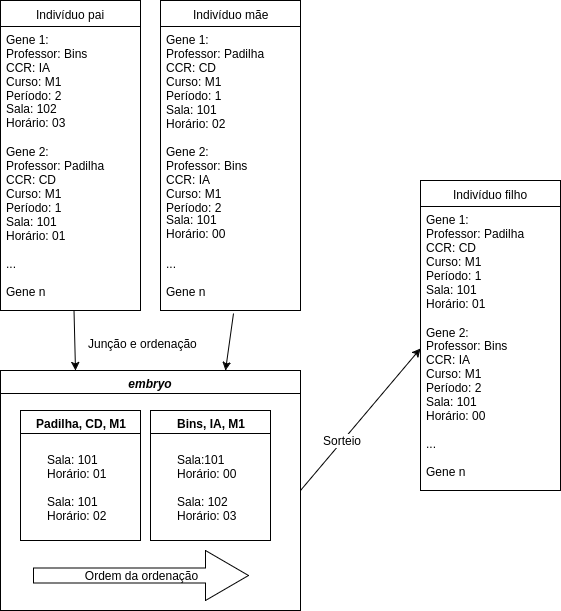
\includegraphics[width=0.7\textwidth]{cross.png}
\end{figure}

Um exemplo simplório de cruzamento é apresentado na Figura \ref{fig:cross} (cabe destacar que na imagem são apresentadas somente as informações necessárias para a explicação). Nele, temos um indivíduo pai e um indivíduo mãe, cada um com uma sequência de genes. Conforme apresentado anteriormente, o passo inicial da função de cruzamento é realizar o agrupamento na estrutura \emph{embryo} dos pares sala e horário do indivíduo pai e do indivíduo mãe que apresentam a mesma tripla professor, componente curricular e curso. No exemplo da Figura \ref{fig:cross} percebe-se que para a tripla Padilha, CD, M1 têm-se os pares sala e horário $(101, 01)$ e $(101, 02)$ e para a tripla Bins, IA, M1 têm-se os pares $(101, 00)$ e $(102, 03)$. Para o exemplo, a ordenação apresenta o CCR CD antes do CCR IA, pois, conforme apresentado, CD apresentava um número menor de períodos. Após a montagem de \emph{embryo} são realizados os sorteios para tomada dos genes que irão compor o cromossomo do indivíduo filho. No exemplo é apresentado no indivíduo filho o resultado de um possível sorteio, no qual temos que o indivíduo filho herdou genes do pai e da mãe.

\section{Mutação dos indivíduos}

A implementação da mutação pode ser encontrada em \emph{mutate()} de \emph{main.cpp}. Tal função é executada após o cruzamento de dois indivíduos e ocorre seguindo a probabilidade de mutação estabelecida no parâmetro constante \textsc{mutation\_rate}.

A função \emph{mutate()} recebe um indivíduo candidato à sofrer uma mutação e constrói uma estrutura que armazena os horários atualmente livres dentre as salas de aula dadas na entrada do problema. Então, itera pelos horários alocados no indivíduo sendo analisado e, ao ser encontrada uma sala de aula com horário disponível e de mesmo curso (e.g. V1...) que o horário sendo considerado no momento, sorteia um horário dentre os disponíveis e realiza a troca de sala e horário no cromossomo do indivíduo.

\section{Parâmetros utilizados na execução do algoritmo}

No total, quatro parâmetros constantes (definido em \emph{main.cpp}) são utilizados ao longo do algoritmo, sendo eles:

\begin{enumerate}
    \item \textsc{population\_size}: representa o tamanho da população;
    \item \textsc{mutation\_rate}: representa a taxa de mutação, a qual varia de $0$ a $100$;
    \item \textsc{max\_generations}: representa o número máximo de gerações pelas quais o algoritmo será executado, caso os demais critérios de parada não sejam satisfeitos antes;
    \item \textsc{max\_unmodified\_generations}: representa o número máximo de gerações sem alteração de \textit{fitness}, considerado como um dos critérios de parada do algoritmo.
\end{enumerate}

\section{Resultado final}

Nos testes realizados observou-se que o algoritmo implementado se comporta conforme esperado e atendeu ao propósito ao qual foi desenvolvido, consistindo em um algoritmo genético para cálculo da tabela de horários dos Componentes Curriculares do curso de Ciência da Computação da UFFS. Ademais, foi observado que na maioria das execuções a \textit{fitness} das populações geradas se mostrou não decrescente e convergiu rapidamente.

% \bibliographystyle{sbc}
% \bibliography{sbc-template}

\end{document}